Discussing the results of experiments. PUT DATASET INSIDE HERE

\section{Aspect classification}

\subsection{BERT fine-tuning}
Due to their size (and the subsequent large amount of data stored in the parameters), it is hard to carry out probing on LLMs, and, due the fact that they appeared recently, there has been less time to develop probing techniques, hence I decided to train a smaller model of the BERT \citep{devlin2019bert} family. These require more data to fine-tune than LLMs, and hence I used the fine-tuned Llama model to generate more training data in a technique known as knowledge distillation (KD). Knowledge distillation involves using a larger 'teacher' model to train a smaller 'student' model, often reaching the same or similar accuracy with a significantly smaller model. While not being able to probe the larger Llama model, smaller models are still an interesting artefact to consider and 

Furthermore, the complexity of larger LMs (especially those trained for generation rather than sequence classification (CHECK THIS!!!!)) means that their embedding space is noisier than smaller models that have been fine-tuned. This makes it harder to do the sort of probing described in later in this chapter.


\subsection{Aspect latent space}
Figure \ref{fig:fine-tuned_aspect_latent_space} provides a visualization of the \texttt{[CLS]} token embedding of verb-sentence pairs in the training set, together with their aspect label, from which several interesting observations can be made. For instance, it is interesting to note the positioning of \texttt{habitual} instances between \texttt{state} and \texttt{activity}, which accurately captures their semantics as somewhere between the more generic, non-episodic state and activities, denoting "an event [that] has not necessarily ended and may be ongoing at Document Creation Time (DCT)" \citep{umr}.

\begin{figure}
    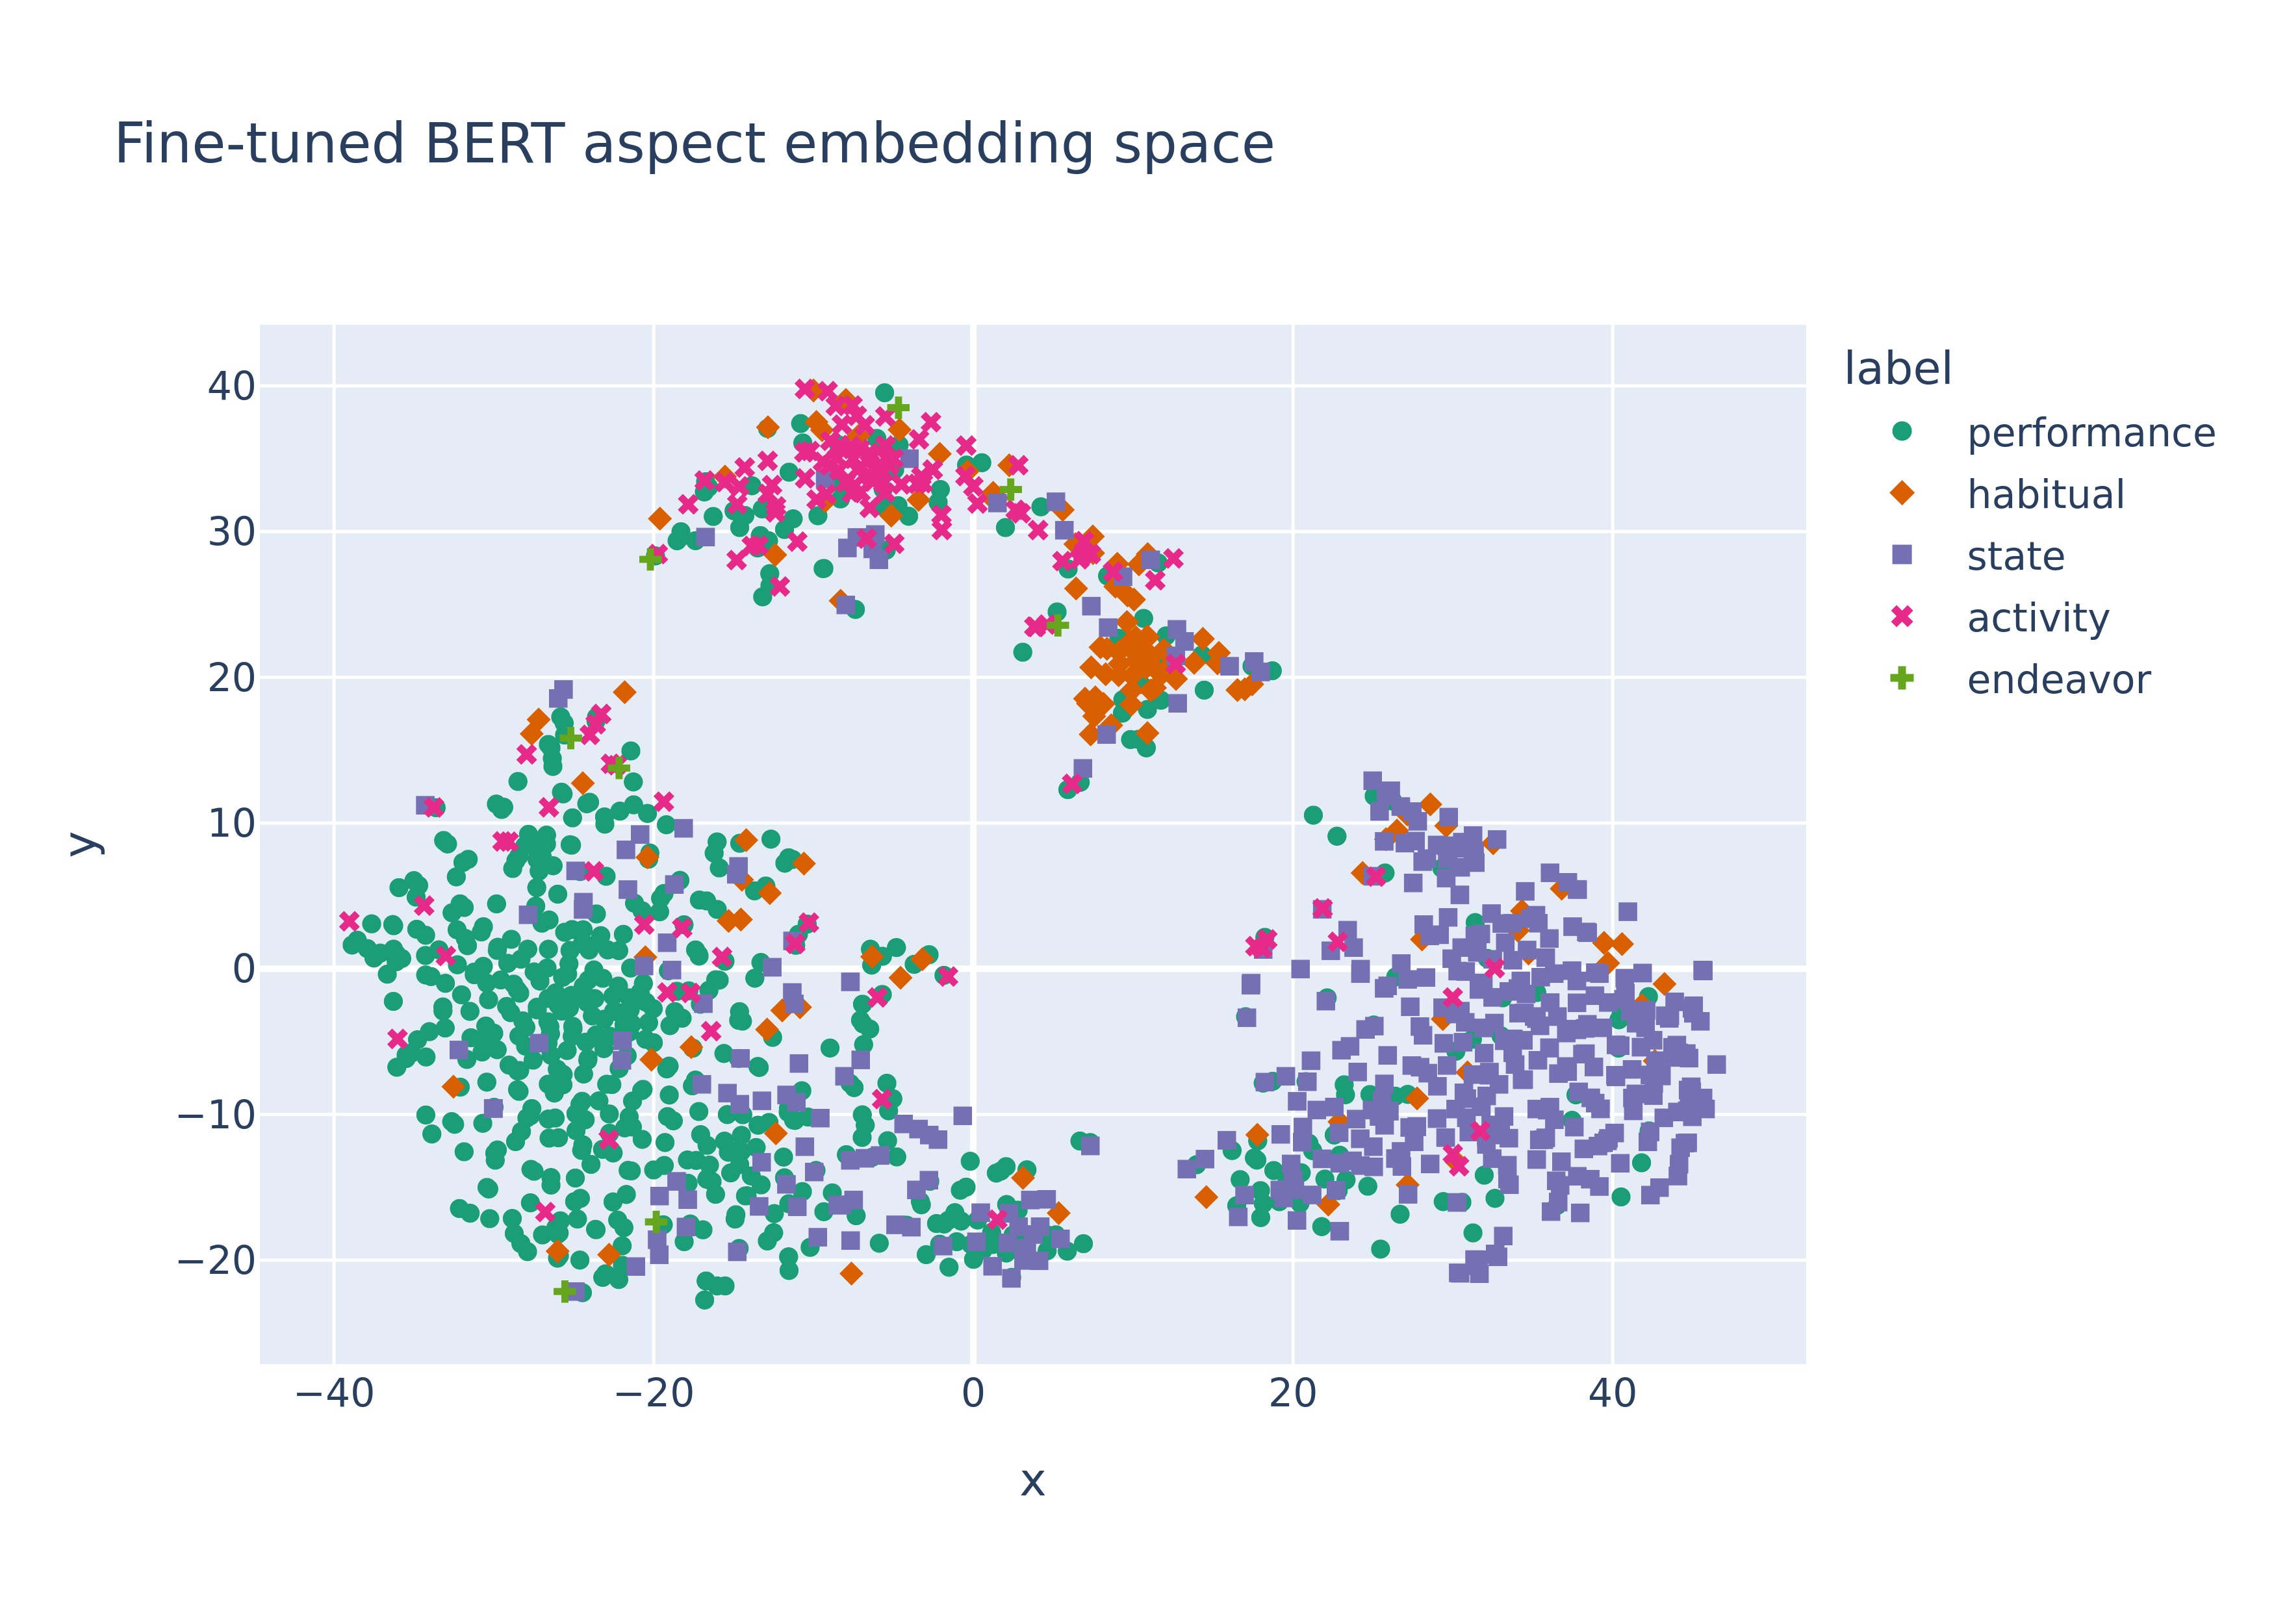
\includegraphics[width=\textwidth]{img/aspect_latent_space.jpeg}
    \caption{\texttt{[CLS]} embedding space of a BERT model fine-tuned on English verbs annotated for aspect in context, reduced to 2 dimensions by t-SNE.}
    \label{fig:fine-tuned_aspect_latent_space}
\end{figure}


\subsection{Multilingual BERT fine-tuning}
Since the LLM annotator Llama 3 can only be used in English, it is only possible to make training data in English. Luckily, however, there are multilingual models which can be trained with data using one language and then be used with languages other than that of the training data. I wanted to verify the performance of different models transferred to other languages and therefore needed a way of obtaining target labels for languages other than English.

I therefore trained a WHICH MODEL using WHICH DATASET annotated by the fine-tuned Llama 3 model and applied. The choice for this particular dataset was the availability of word-level alignments, a rarity in parallel corpora (IS THIS TRUE), meaning once a verb has been identified in the English sentence and given a particular aspect class, it is easy to find the corresponding verb in the other language. I only included sentences where the corresponding word in the other language is also a verb, since I wish to focus on verb phrases rather than general event classification.

In order to check the performance of this 

Get results in English and results in French

ENTER RESULTS

Hence, it is clear that the result is worse than in English, as is to be expected, however still significantly higher than chance.

\subsubsection{Russian aspect system}
As explained in \ref{sec:asp_in_slav_lang}
\subsubsection{Verb of motion clustering}
Unlike in English, almost all Russian imperfective verbs of motion have both a telic and an atelic counterpart. The former is used to describe a motion with a destination, the latter for one without.

\begin{exe}
    \ex Ja \emph{SHel} v SHkolu. (I was walking to school.)
    \ex Ja \emph{hodil} po parku. (I was walking around the park.)
\end{exe}

In UMR, events with no end goal are PROTOTYPISED? by activity, whereas telic events reaching completion are annotated with \texttt{performance}. We can verify that the model also makes this distinction HOW.

this empirically using the 

Using this we can 

\subsubsection{Prefix clustering}
An interesting application of this fine-tuned model is the 

\section{Aspectual ambiguity}
\subsection{Sentence-level ambiguity}
DOES ENTROPY CORRELATE WITH AMBIGUITY PREDICTION??
It is well known that LMs are often too confident of their predictions, even when wrong INSERT CITATION HERE

The first question that is interesting to ask (CHANGE DIESE FORMULIERUNG) is whether there is a correlation between the uncertainty of the aspect classification model and the output of the aspect ambiguity model, i.e. does a (supposed) ambiguous aspect reading of a sentence-verb pair correlate with uncertainty in the former's output. In order to quantify I take the concept of entropy and apply it to this case with the following formula:

$$H_{aspect} = - \sum_{i=1}^{\#AspClass}p(x_i)log(p(x_i))$$

In this way, higher uncertainty (i.e. a more balanced probability across all classes) leads to a higher $H_{aspect}$ value. It must be noted that this value is not comparable with models outputting a different number of classes (such as the traditional Vendlerian classification with 4), or indeed with different aspect classification systems (IS THIS TRUE??), however it serves the purpose for use to compare between languages (REWORD).

Using this value it is possible to calculate a correlation coefficient. The measure used was the point-biserial correlation coefficient, a metric mathematically equivalent to Pearson's correlation coefficient, however specialised for the case of one binary and one continuous variable. It is calculated thus:

$$ENTER BPS EQUATION$$


\subsection{Verb-level ambiguity}

\subsection{Language-level ambiguity: Cross-linguistic comparison}
